\nl{В космологии есть несколько способов определения расстояний (Hogg1999).  }
%Здесь и далее 
Для описания расстояний между объектами в системе источник - линза - наблюдатель используется понятие расстояния углового диаметра (\textit{angular diameter distance}). Оно определяется следующим образом:
%(\cite{distance_measures}, в данной публикации приведены и другие способы определения расстояния, используемые в космологии):

\begin{equation}\label{ang_dia_dist}
D_{A}\left(z_{1}, z_{2}\right)=\frac{c}{1+z_{2}} \int_{z_{1}}^{z_{2}} \frac{d z}{H_{0} \sqrt{\Omega_{m}\left(1+z\right)^{3}+\Omega_{\Lambda}}},
\end{equation}
где $z_1, z_2$ - красные смещения  соответственно линзы и источника. В данной работе мы рассматриваем плоскую Вселенную со следующими параметрами: $H_0=70$ (км/с)/Мпк, $\Omega_m=0.3, \Omega_\Lambda=0.7$.
%Выбор этих параметров обусловлен рассмотрением здесь и далее модели \textit{плоской Вселенной}.

Источники: (\cite{suyu2010}), (\cite{timedelaycosmography})

Важным свойством гравитационного линзирования является возможность формирования нескольких изображений одного и того же источника. Свет, преломляющийся в поле точечной линзы с гравитационным потенциалом $\Psi(\boldsymbol{\theta})$, распространяется от источника до наблюдателя за время

\begin{equation}\label{tau}
\tau(\boldsymbol{\theta}, \boldsymbol{\beta})=\frac{1}{c} \frac{D_{d} D_{s}}{D_{d s}} (1+z_1) \cdot \Phi(\boldsymbol{\theta},\boldsymbol{\beta}),
\end{equation}

\begin{equation}\label{fi}
\textrm{где} \ \Phi(\boldsymbol{\theta},\boldsymbol{\beta}) =  \left[\frac{1}{2}(\boldsymbol{\theta}-\boldsymbol{\beta})^{2}-\Psi(\boldsymbol{\theta})\right].
\end{equation}

%где $\boldsymbol{\theta}$ и $\boldsymbol{\beta}$ -- положения (в угловых единицах) соответственно изображения и источника (см. Рис.\ref{fig:gravlensfig}). 

Множитель $\Phi(\boldsymbol{\theta},\boldsymbol{\beta})$ называется \textit{потенциалом Ферма}. Первое слагаемое означает геометрическую задержку, так как траектория, вдоль которой распространеняется свет, удлиняется, и, как следствие, увеличивается время его распространения относительно прямой линии. Второе слагаемое - гравитационная задержка, также известная как эффект Шапиро (\cite{shapiro1964}), так как в соответствии с ОТО время около гравитирующих тел идет “медленнее”. В соответствии с принципом Ферма изображения формируются там, где $\nabla \tau(\boldsymbol{\theta}, \boldsymbol{\beta}) = \nabla \Phi(\boldsymbol{\theta}, \boldsymbol{\beta}) = 0 $ (\cite{schneider1985}). $\Phi(\boldsymbol{\theta},\boldsymbol{\beta})$ можно представить как пространственно-переменный показатель преломления линзы. Следовательно, возможно появление нескольких изображений  одного и того же источника (то есть возможно несколько значений $\boldsymbol{\theta}$ для одного положения источника $\boldsymbol{\beta}$). Так как отдельные лучи света от источника, дошедшие до наблюдателя, отклоняются под разными углами, геометрические задержки для них различны (см. Рис. \ref{fig:timedelayorigin}).

(!) оставить? \nl{мне кажется, что лучше убрать}
%schneider 2006 страница 54
Существует альтернативный подход, в котором рассматриваются волновые фронты от различных положений изображений (\cite{kayzerrefsdal1983}). Результат этого подхода в точности совпадает с полученным выше. Эта идея также проиллюстрирована на Рис. \ref{fig:timedelayorigin}.

%We see images at extrema of the virtual time delay surface (164 page)
%\cite{blandfordnarayan1986}
%https://ui.adsabs.harvard.edu/abs/1986ApJ...310..568B/abstract

\begin{figure}[h]
    \centering
	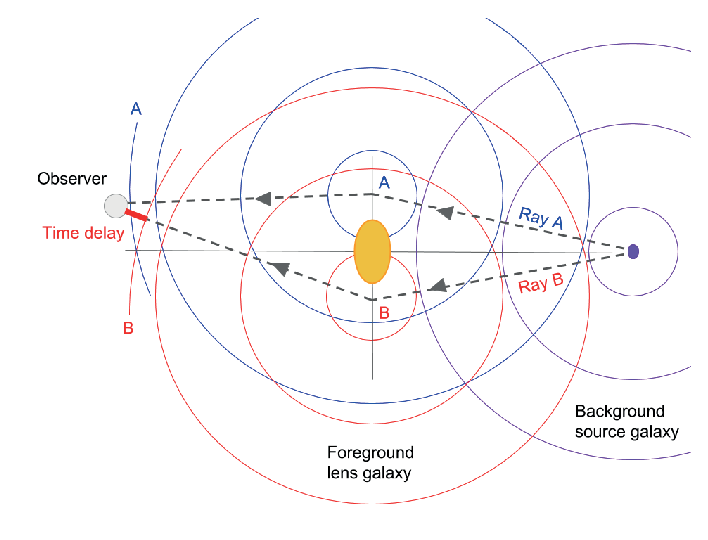
\includegraphics[scale=1.0]{pics/timedelayorigin.eps}
	\caption{Схематичная иллюстрация возникновения "геометрического" слагаемого в выражении для временной задержки. \label{fig:timedelayorigin} }
   \end{figure} 


Введём обозначение:
 
\begin{equation}\label{dDt}
D_{\Delta t} = \frac{D_{d} D_{s}}{D_{d s}} (1+z_1) 
\end{equation}

Нетрудно увидеть, что величина $D_{\Delta t}$ (которая иногда называется \textit{расстоянием временной задержки} (time-delay distance) обратно пропорциональна $H_0$, что видно из \eqref{ang_dia_dist}. Важно отметить множитель (1+$z_1$), который возникает из-за расширения Вселенной (временная задержка "происходит" на красном смещении $z_1$). Можно упростить уравнение \eqref{tau} следующим образом:

\begin{equation}\label{ef}
\tau(\boldsymbol{\theta}, \boldsymbol{\beta})=\frac{D_{\Delta t}}{c} \Phi(\boldsymbol{\theta},\boldsymbol{\beta}) \propto \frac{1}{H_0}\Phi(\boldsymbol{\theta},\boldsymbol{\beta}).
\end{equation}

Непосредственно $\tau(\boldsymbol{\theta}, \boldsymbol{\beta})$ не поддаётся измерению. Но зато можно измерить разницу этих величин для различных изображений.

\begin{equation}\label{dt}
\Delta \tau_{AB} = \tau(\boldsymbol{\theta}_A, \boldsymbol{\beta}) - \tau(\boldsymbol{\theta}_B, \boldsymbol{\beta}) \propto \frac{1}{H_0}\Delta \Phi_{AB}.
\end{equation}

%Knowledge of the lens mass distribution is of vital importance to the success of this cosmological inference: Equation 3 shows that the time delay distance is likely to be comparably sensitive to uncertainty in the predicted Fermat potential as it is to the measured time delay itself. More concentrated mass distributions with steeper density profiles produce longer time delays leading to shorter inferred time delay distances, and thus larger inferred values of H0 (Wucknitz, 2002; Kochanek, 2002; Suyu, 2012).

%Both α(θ) and ψ(θ) can be predicted given a model for the mass distribution of the lens.

Если смоделировать линзирующий потенциал $\Psi(\boldsymbol{\theta})$ и положение источника $\boldsymbol{\beta}$ (которое не наблюдается) и на основе этих данных рассчитать $\Delta \Phi_{AB}$, то можно использовать гравитационно линзирующие системы для вычисления постоянной Хаббла $H_0$ и других космологических параметров, например, безразмерные плотности материи $\Omega_m$ и тёмной энергии $\Omega_{\Lambda}$ (см. \eqref{ang_dia_dist}). Но зависимость $D_{\Delta t}$ от $H_0$ наиболее сильная, поэтому дальнейшее исследование посвящено именно этому параметру.

Отметим, что распределение массы в линзы подвержено ряду вырождений, самым существенным из которых является так называемое \nl{поискать название в русско-язычной лит-ре}"вырождение масса-плоскость" (mass-sheet degeneracy). Данное вырождение заключается в том, что существует такое преобразование модели распределения массы в линзе, при котором наблюдаемые величины - положения изображений источника, относительные усиления, видимые звездные величины (наблюдаемый поток) - остаются прежними, в то время, как временные задержки могут испытывать серьёзные изменения (\cite{falco1985}). Для снятия данного вырождение необходимо привлечение дополнительной информации о потенциале линзы. Например, моделированием динамики звёзд в галактике-линзе или изучением среды вдоль луча зрения
(\cite{suyu2010}).
 
Весь формализм выше описывает простую модель, в которой вся гравитирующая масса расположена в одной плоскости. Моделирование настоящих гравитационно линзирующих систем гораздо сложнее, но соотношение \eqref{dt} так или иначе возникает в ходе вычислений, поэтому зависимость от космологических параметров сохраняет свою форму. \nl{зачем этот абзац? при моделировании линзы все до сих пор пользуются приближением плоской линзы}

Для определения постоянной Хаббла по временной задержке между изображениями, блеск источника должен быть переменным. Разные его изображения, возникающие в результате гравитационного линзирования, будут изменять свой блеск также, как и источник, но с некоторой задержкой по времени. Измеряя временную задержку между изображениями одного и того же источника, можно получить значение постоянной Хаббла. Идея использования именно линзированных сверхновых для оценки $H_0$ была впервые предложена Сьюром Рефсдалом в 1964 году (\cite{refsdal1964}). \nl{повтор введения}